\documentclass[11pt]{article}
\usepackage{icmlko}
\begin{document}

\title{유보를 늘릴 길을 다 걸어 봤다 --- 이제 남은 것은 수집뿐이다}
\author{월드모델 실험실}
\date{노트 373 · 2026년 8월 1일}
\maketitle

\begin{abstract}
노트 352가 이 창의 물음을 세웠다 --- \emph{판 55쌍 중 33쌍은 순서를 못
가리고, 그 폭은 유보 행수가 정한다.} 그 뒤 스물한 편이 여러 도메인에서
유보를 늘리려 했다. \textbf{여기서 지도를 그린다.} 얇은 여섯 도메인
전부에서 길이 막혀 있고, \textbf{여섯 가지 이유가 다 다르다} --- 아이돌은
라벨이 없고(107건 중 대체 필드가 25 중 1건, 원천은 사이트가 AI/ML 수집을
금지한다), 팝업은 남은 247건이 \emph{무신호}이고(노트 360), 펀딩은
\textbf{버림이 0\%}라 이미 다 쓰고 있고, 시장팝업은 노트 354가 규칙으로
44행을 회수한 뒤 쓸 만한 것이 19건(2025+ 7)만 남았고, 도서는 전자책
153건이 근거를 갖고 빠졌고(노트 35 · 253), 만화는 KR 322건의 \emph{부호가
뒤집힌다}(노트 372). \textbf{분석으로 갈 수 있는 데까지 갔다.} 남은 길은
하나뿐이다 --- \textbf{실제로 세어서 모으는 것}. 팝업 실측 41행 · 최근
펀딩 · 라벨 있는 아이돌 데뷔.
\end{abstract}

\section{지도}

\begin{center}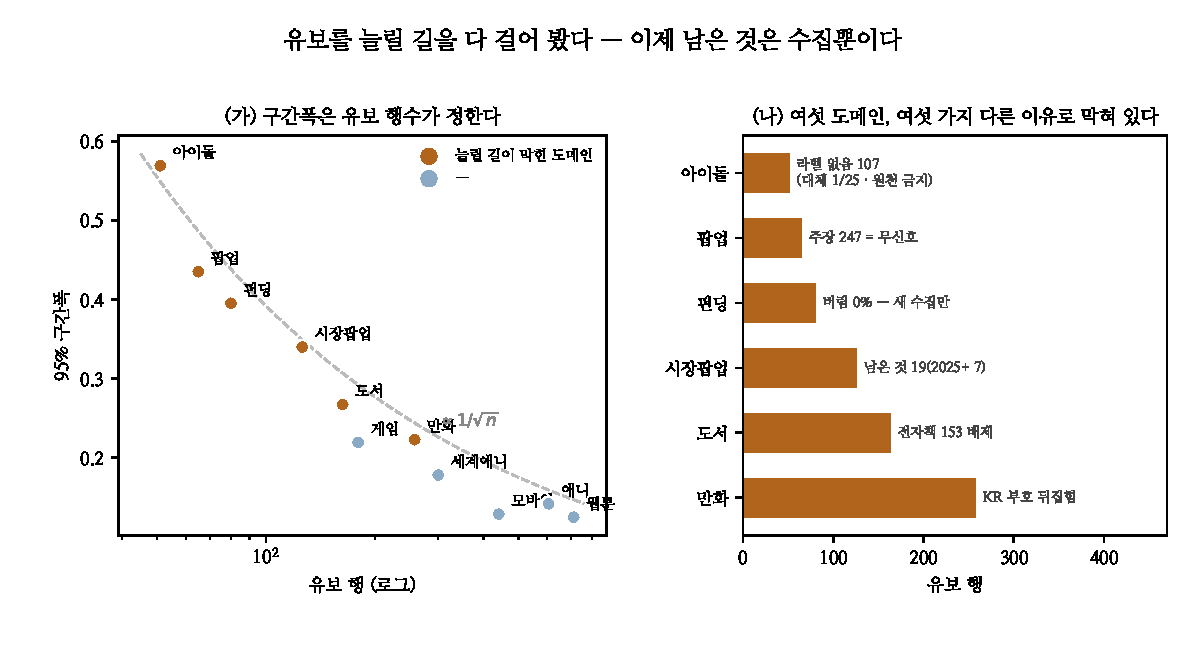
\includegraphics[width=\linewidth]{figs/head.pdf}\end{center}

\begin{center}\small
\begin{tabular}{lrrl}
\hline
도메인 & 유보 & 가중 & 왜 못 늘리나 \\
\hline
아이돌 & 51 & 1.7\% & 레코드 282 중 \texttt{chodong} 없음 \textbf{107}(2025+ 25).
  대체 필드 \\
 & & & \texttt{chart\_peak} 는 \texttt{chodong} 과 $-0.811$ 로 세지만 그 25 중
  \textbf{1건}뿐. \\
 & & & 원천(써클차트)은 사이트가 \textbf{AI/ML $\cdot$ TDM 수집을 금지}한다 \\
팝업 & 65 & 2.2\% & 레코드 376 중 실측 계수 91 · 주장 \textbf{247}. 주장은
  수준이 \\
 & & & 아니라 \textbf{무신호}다(노트 360 --- 2025년 $\rho=+0.0070$) \\
펀딩 & 80 & 2.7\% & 레코드 400 $=$ 축 400. \textbf{버림 0\%} --- 이미 다 쓴다 \\
시장팝업 & 126 & 4.2\% & 미사용 398 중 라벨 $\cdot$ 기간이 있는 것 \textbf{19}
  (2025+ 7). \\
 & & & 노트 354가 규칙으로 44행을 회수한 뒤 남은 것이다 \\
도서 & 163 & 5.5\% & 전자책 153 --- 라벨과 $-0.81$, 판형 $\cdot$ 무게 0\%
  (노트 35 · 253) \\
만화 & 258 & 8.7\% & KR 322 $\cdot$ CN 19 가 더 있으나 \textbf{부호가 뒤집힌다}
  (노트 372) \\
\hline
\end{tabular}
\end{center}

\textbf{여섯 도메인, 여섯 가지 다른 이유다.} 하나의 병이 아니라 각자
다른 벽에 부딪혔고, 그 벽이 무엇인지는 이제 다 적혀 있다.

\section{길이 다르다는 것이 결과다}

이 창에서 유보를 늘리려 한 시도와 그 끝은 이랬다.

\begin{center}
\begin{tabular}{lll}
\hline
노트 & 무엇을 했나 & 끝 \\
\hline
353 & 아이돌 유보 $25 \to 51$ & \textbf{넣음}(구간폭 $0.757 \to 0.556$) \\
354 & 시장팝업 MKT2 44행 & \textbf{넣음}(유보 $104 \to 126$) \\
357 & 팝업 계수 필터 풀기 & 기준이 안 섞인다 --- 기각 \\
358 & 팝업 등급 필터 풀기 & \textbf{넣음}(유보 $59 \to 65$) \\
360 & 팝업 주장 라벨 정규화 & 무신호 --- 기각 \\
365 · 370 & 만화 258행 & \textbf{넣음}(0행 $\to$ 258, 열한 번째 도메인) \\
372 & 만화 KR/CN 583행 & 부호 뒤집힘 --- 기각 \\
\textbf{373} & \textbf{나머지를 다 훑음} & \textbf{남은 길 없음} \\
\hline
\end{tabular}
\end{center}

\textbf{넷은 들어갔고 셋은 막혔고, 이제 훑을 것이 없다.} 들어간 넷이
못 가리는 쌍을 67\%(30/45)에서 60\%(33/55)로 옮겼다 --- 도메인이 하나
늘면서도 비율이 내려갔다.

\section{그러니 다음은 수집이다}

\begin{itemize}
\item \textbf{팝업 실측 41행}(노트 360). 학습 24행을 65행으로 만들면 노트
276의 전용 축 넷이 짝 규약 아래서 산다(노트 359의 셈). 그리고 팝업은
이 실험실의 결정을 다섯 번 연속 내린 수다(노트 366).
\item \textbf{최근 펀딩.} 유보 80은 자료를 버려서가 아니라 2025년 이후
프로젝트가 그만큼뿐이라 그렇다. \textbf{버림 0\%인 유일한 도메인}이고,
그래서 수집이 그대로 유보가 된다.
\item \textbf{라벨 있는 아이돌 데뷔.} 2025년 이후 25건이 초동 없이 있다.
써클차트는 막혔으니 다른 출처가 필요하다.
\end{itemize}

\textbf{그리고 수집은 정렬을 적어 둔다}(노트 365). 인기순 · 베스트셀러 ·
계수 방법 --- 세 도메인에서 수집 정렬이 과제를 정했다. 무엇으로 정렬해
모았는지를 도메인 문서에 남긴다.

\section{규약에 더하는 줄}

\begin{itemize}
\item \textbf{``유보를 늘리자''는 도메인마다 다른 일이다.} 여섯이 여섯
가지 이유로 막혔다 --- 하나를 뚫은 방법이 다음에 안 통한다.
\item \textbf{원천의 이용 조건을 먼저 본다.} 써클차트 경로는 사이트가
AI/ML $\cdot$ TDM 을 금지해 닫혀 있다. \emph{할 수 있느냐}보다 \emph{해도
되느냐}가 먼저다.
\item \textbf{버림 0\%는 좋은 신호가 아니라 천장 신호다}(펀딩) --- 더
짜낼 것이 없다는 뜻이다.
\end{itemize}

\section{남은 것}

\begin{center}
\begin{tabular}{ll}
\hline
갈래 & 지금 아는 것 \\
\hline
\textbf{팝업 실측 41행} & 수집. 전용 축 넷이 살아난다 \\
\textbf{최근 펀딩} & 수집. 버림 0\% 라 모으는 대로 유보가 된다 \\
아이돌 라벨 25건 & 써클차트는 막혔다. 다른 출처 \\
KR 웹툰을 웹툰 도메인으로 & 노트 372. 제목 정합부터(로마자) \\
세계애니 눈금 & 노트 369. 합친 백분위가 12/12 로 올렸다 \\
\hline
\end{tabular}
\end{center}

\end{document}
